\documentclass[a4paper]{article}
\usepackage{graphicx} % Required for inserting images
\usepackage{todonotes}
\usepackage{geometry}
\usepackage{listings}
\geometry{a4paper, top=3cm, bottom=3cm, left=3.5cm, right=3.5cm} % heightrounded, bindingoffset=5mm}

\title{Progetto Basi di Dati 2024-25 \\
“FANTASANREMO” \\
Parte III}
\author{Team 35
	\\
	\and Alessio Molinas 5339413\\Ettore Romano 5644926}
\date{}

\begin{document}

\maketitle


\section{Progettazione Fisica\\}

\subsection{CARICO DI LAVORO\\}

\subsubsection{Q1 - QUERY CON SINGOLA SELEZIONE E NESSUN JOIN\\}

\paragraph*{LINGUAGGIO NATURALE \\} 


\todo[inline]{Seleziona tutte le informazioni degli artisti dalla tabella artisti\_cl il cui nome è esattamente 'Ana'}

\paragraph*{SQL \\}

%\todo[inline]
\begin{lstlisting}[language=SQL]
SELECT *
FROM artisti_cl
WHERE nome = 'Ana';
\end{lstlisting}



\subsubsection{Q2 - QUERY CON CONDIZIONE DI SELEZIONE COMPLESSA E NESSUN JOIN\\}

\paragraph*{LINGUAGGIO NATURALE\\}

\todo[inline]{Seleziona tutte le informazioni degli artisti dalla tabella artisti\_cl che si chiamano Ana e sono nati dopo il 1° gennaio 1992.}

\paragraph*{SQL \\}

\begin{lstlisting}[language=SQL]
SELECT *
FROM artisti_cl
WHERE nome = 'Ana' AND dataNascita >= DATE '1992-01-01';
\end{lstlisting}


\subsubsection{Q3 - QUERY CON ALMENO UN JOIN E ALMENO UNA CONDIZIONE DI SELEZIONE\\ }

\paragraph*{LINGUAGGIO NATURALE\\}

\todo[inline]{Seleziona tutte le informazioni relative alle leghe chiamate 'Anthony', insieme alle squadre che vi partecipano e ai dettagli della partecipazione a quelle leghe}

\paragraph*{SQL \\}

%\todo[inline]{Riportare in questa sezione l’interrogazione del carico di lavoro con almeno un join e almeno una condizione di selezione, in SQL}
\begin{lstlisting}[language=SQL]
	SELECT * FROM leghe_cl l
	JOIN partecipazione_leghe_cl pl ON l.codLega = pl.codLega
	JOIN squadre_cl s ON pl.codSquadra = s.codSquadra
	WHERE l.nome = 'Anthony';
\end{lstlisting}


\subsection{1D-PROGETTO FISICO\\}

\todo[inline]{Riportare nella seguente tabella l’elenco degli indici che si intendono creare per: (1) ciascuna query del carico di lavoro individualmente; (2) l’insieme delle query del carico di lavoro, motivando opportunamente, in modo sintetico, le scelte effettuate}


\begin{center}
\begin{footnotesize}
\begin{tabular}{|c|c|p{2cm}|p{2cm}|p{5cm}|}
\hline
{\bf Id query} & {\bf Relazione} & \parbox{2cm}{\bf Chiave di ricerca} & \parbox{2cm}{\bf Tipo (ordinato/hash, clusterizzato/non clusterizzato)} & \parbox{5cm}{\bf Motivazione} \\
\hline
Q1 & artisti & nome & ordinato e clusterizzato &  Visto il numero frequente di query sull'attributo nome (non UNIQUE) potrei optare per la clusterizzazione\\
Q2 & artisti & nome, dataNascita & ordinato e clusterizzato & Devo escludere indice hash perchè è prevista ricerca per range sulla data nascita. Opterei per un indice composto per facilitare sia la query precedente che quella corrente\\
Q3 & leghe, partecipazione\_leghe, squadre & leghe.nome & ordinato & Oltre all'indice su leghe.nome, introdurrei degli indici sulle chiavi utilizzate per eseguire le join. Questi permettono di utilizzare algoritmi di join come l'indexed nested loop.\\
\hline
\end{tabular}
\end{footnotesize}
\end{center}



\begin{center}
\begin{footnotesize}
\begin{tabular}{|p{6.5cm}|p{6.5cm}|}
\hline
\parbox{5cm}{\bf Schema fisico complessivo per il carico di lavoro} &  \parbox{5cm}{\bf Motivazione} \\
\hline
- indice ordinato e clusterizzato su (nome, dataNascita), tabella artisti& Ricerca per nome con uguaglianza e dataNascita per range (anche per ricerca attraverso solo per nome) \\
- indice ordinato su nome, tabella leghe& Ricerca per nome\\
\hline
\end{tabular}
\end{footnotesize}
\end{center}

\subsection{1G-ANALISI PIANI DI ESECUZIONE SCELTI DAL SISTEMA\\}


\subsubsection{Q1 - QUERY CON SINGOLA SELEZIONE E NESSUN JOIN\\}

\paragraph*{PIANO DI ESECUZIONE SCELTO DAL SISTEMA PRIMA DELLA CREAZIONE DELLO SCHEMA FISICO\\}

\todo[inline]{Seq Scan on artisti\_cl as artisti\_cl Filter: ((nome)::text = 'Ana'::text)}


\paragraph*{PIANO DI ESECUZIONE SCELTO DAL SISTEMA DOPO DELLA CREAZIONE DELLO SCHEMA FISICO\\}

\todo[inline]{Index Scan using idx\_artisti\_cl\_nome\_datanascita on artisti\_cl as artisti\_cl Index Cond: ((nome)::text = 'Ana'::text)}

\paragraph*{CONFRONTO TRA I DUE PIANI\\}

\todo[inline]{Riportare nella seguente tabella i tempi di esecuzione per i piani ottenuti prima e dopo la creazione dello schema fisico complessivo, giustificando i piani e i tempi ottenuti}


\begin{center}
\begin{footnotesize}
\begin{tabular}{|p{3cm}|p{3cm}|p{7cm}|}
\hline
\parbox{3cm}{\bf Tempo esecuzione PRIMA} & \parbox{3cm}{\bf Tempo esecuzione DOPO} &  \parbox{7cm}{\bf Motivazione} \\
\hline
00:00:00.153 & 00:00:00.054 & Viene utilizzato l'indice composto per la ricerca per nome (senza eseguire confronti sulla data)  \\
\hline
\end{tabular}
\end{footnotesize}
\end{center}

\subsubsection{Q2 - QUERY CON CONDIZIONE DI SELEZIONE COMPLESSA E NESSUN JOIN\\}

\paragraph*{PIANO DI ESECUZIONE SCELTO DAL SISTEMA PRIMA DELLA CREAZIONE DELLO SCHEMA FISICO\\}

\todo[inline]{Seq Scan on artisti\_cl as artisti\_cl
	Filter: ((datanascita  $\geq$ '1992-01-01'::date) AND ((nome)::text = 'Ana'::text))}

\paragraph*{PIANO DI ESECUZIONE SCELTO DAL SISTEMA DOPO DELLA CREAZIONE DELLO SCHEMA FISICO\\}

\todo[inline]{Index Scan using idx\_artisti\_cl\_nome\_datanascita on artisti\_cl as artisti\_cl
 Index Cond: (((nome)::text = 'Ana'::text) AND (datanascita $\geq$ '1992-01-01'::date))}

\paragraph*{CONFRONTO TRA I DUE PIANI\\}

\todo[inline]{Riportare nella seguente tabella i tempi di esecuzione per i piani ottenuti prima e dopo la creazione dello schema fisico complessivo, giustificando i piani e i tempi ottenuti}


\begin{center}
\begin{footnotesize}
\begin{tabular}{|p{3cm}|p{3cm}|p{7cm}|}
\hline
\parbox{3cm}{\bf Tempo esecuzione PRIMA} & \parbox{3cm}{\bf Tempo esecuzione DOPO} &  \parbox{7cm}{\bf Motivazione} \\
\hline
00:00:00.079 & 00:00:00.052 & Viene utilizzato l'indice composto per ricerca con nome uguale ad un valore e data con un range \\
\hline
\end{tabular}
\end{footnotesize}
\end{center}



\subsubsection{Q3 - QUERY CON ALMENO UN JOIN E ALMENO UNA CONDIZIONE DI SELEZIONE \\}

\paragraph*{PIANO DI ESECUZIONE SCELTO DAL SISTEMA PRIMA DELLA CREAZIONE DELLO SCHEMA FISICO\\}

\todo[inline]{
	- Hash Inner Join \\
	- Hash Cond: (s.codsquadra = pl.codsquadra) \\
	- Seq Scan on squadre\_cl as s \\
	- Hash \\
	- Hash Inner Join \\
	- Hash Cond: (pl.codlega = l.codlega) \\
	- Seq Scan on partecipazione\_leghe\_cl as pl \\
	- Hash \\
	- Seq Scan on leghe\_cl as l \\
	- Filter: ((nome)::text = 'Anthony'::text) \\
	}

\paragraph*{PIANO DI ESECUZIONE SCELTO DAL SISTEMA DOPO DELLA CREAZIONE DELLO SCHEMA FISICO\\}

\todo[inline]{
	- Hash Inner Join \\
	- Hash Cond: (s.codsquadra = pl.codsquadra) \\
	- Seq Scan on squadre\_cl as s \\
	- Hash \\
	- Hash Inner Join \\
	- Hash Cond: (pl.codlega = l.codlega) \\
	- Seq Scan on partecipazione\_leghe\_cl as pl \\
	- Hash \\
	- Bitmap Heap Scan on leghe\_cl as l \\
	- Recheck Cond: ((nome)::text = 'Anthony'::text) \\
	- Bitmap Index Scan using idx\_leghe\_cl\_nome \\
	- Index Cond: ((nome)::text = 'Anthony'::text) \\
}

\paragraph*{CONFRONTO TRA I DUE PIANI\\}

\todo[inline]{Riportare nella seguente tabella i tempi di esecuzione per i piani ottenuti prima e dopo la creazione dello schema fisico complessivo, giustificando i piani e i tempi ottenuti}


\begin{center}
\begin{footnotesize}
\begin{tabular}{|p{3cm}|p{3cm}|p{7cm}|}
\hline
\parbox{3cm}{\bf Tempo esecuzione PRIMA} & \parbox{3cm}{\bf Tempo esecuzione DOPO} &  \parbox{7cm}{\bf Motivazione} \\
\hline
00:00:00.043 & 00:00:00.052 & Nonostante la creazione di un indice sul nome della lega — testato sia in versione clusterizzata che non — la query non ha ottenuto benefici significativi in termini di performance. Sono stati inoltre effettuati alcuni test con la creazione di indici sui campi utilizzati per le join (i codici delle relazioni), ma anche in questo caso il database ha preferito utilizzare l’hash join, ignorando gli indici disponibili.
 \\
\hline
\end{tabular}
\end{footnotesize}
\end{center}




\section{CONTROLLO DELL’ACCESSO\\}

\subsection{GERARCHIA TRA I RUOLI \\}

\subsubsection{GERARCHIA\\}

\todo[inline]{Riportare in questa sezione la gerarchia che si intende definire tra i quattro ruoli}
La gerarchia scelta è la seguente:
\[
\texttt{admin\_fanta} \rightarrow \texttt{admin\_lega} \rightarrow \texttt{proprietario\_lega} \rightarrow \texttt{utente\_semplice}
\]

\subsubsection{MOTIVAZIONE GERARCHIA}

\todo[inline]{Riportare in questa sezione una motivazione per la gerarchia proposta}
\subsection*{Gerarchia dei ruoli e motivazioni}

La gerarchia dei ruoli nel sistema FantaSanremo è stata progettata seguendo i principi del \textbf{minimo privilegio} e della \textbf{modularità dei compiti}. La struttura gerarchica è la seguente:

\begin{center}
	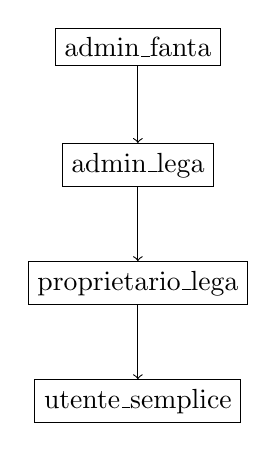
\begin{tikzpicture}[node distance=1.5cm]
		\node (adminfanta) [draw, rectangle] {admin\_fanta};
		\node (adminlega) [draw, rectangle, below of=adminfanta] {admin\_lega};
		\node (proplega) [draw, rectangle, below of=adminlega] {proprietario\_lega};
		\node (utente) [draw, rectangle, below of=proplega] {utente\_semplice};
		
		\draw[->] (adminfanta) -- (adminlega);
		\draw[->] (adminlega) -- (proplega);
		\draw[->] (proplega) -- (utente);
	\end{tikzpicture}
\end{center}

\paragraph{utente\_semplice} È il ruolo con i privilegi minimi, dedicato agli utenti che partecipano al gioco. Può consultare i dati delle leghe, artisti e squadre, ma non modificarli.\\
\textbf{Motivazione:} deve solo accedere ai dati pubblici e non alterare lo stato del sistema.

\paragraph{proprietario\_lega} Questo ruolo rappresenta l’utente che crea e gestisce una propria lega. Ha il diritto di gestire la partecipazione alla lega e modificare i dati della propria squadra.\\
\textbf{Motivazione:} ha responsabilità amministrative limitate alla propria lega.

\paragraph{admin\_lega} Oltre ai privilegi del proprietario di lega, può modificare tutte le leghe, squadre e partecipazioni.\\
\textbf{Motivazione:} è pensato per supervisionare l’intera struttura delle leghe.

\paragraph{admin\_fanta} È il super amministratore del sistema, con pieni privilegi su tutte le tabelle.\\
\textbf{Motivazione:} è responsabile della gestione globale del sistema e delle attività di manutenzione.

\medskip

\noindent
Questa gerarchia consente di:
\begin{itemize}
	\item garantire la \textbf{sicurezza}, evitando accessi non autorizzati a utenti con ruoli minori;
	\item mantenere la \textbf{chiarezza}, grazie all'ereditarietà dei privilegi tra ruoli;
	\item migliorare la \textbf{manutenibilità}, poiché i privilegi possono essere gestiti centralmente tramite i ruoli.
\end{itemize}




\subsection{ASSEGNAZIONE PRIVILEGI SPECIFICI AI RUOLI}

\begin{center}
	\begin{footnotesize}
		\begin{tabular}{|c|p{2.7cm}|p{2.7cm}|p{2.7cm}|p{2.7cm}|}
			\hline
			{\bf Relazione} & \parbox{2.7cm}{\bf Amministratore del FantaSanremo} & \parbox{2.7cm}{\bf Utente semplice} &  \parbox{2.7cm}{\bf Amministratore lega} & \parbox{2.7cm}{\bf Proprietario lega} \\
			\hline
			\texttt{artisti} & ALL PRIVILEGES & SELECT & SELECT & SELECT \\
			\hline
			\texttt{leghe} & ALL PRIVILEGES & - & INSERT, SELECT, UPDATE & INSERT, SELECT \\
			\hline
			\texttt{partecipazione\_leghe} & ALL PRIVILEGES & INSERT, SELECT & INSERT, SELECT, UPDATE & INSERT, SELECT \\
			\hline
			\texttt{squadre} & ALL PRIVILEGES & INSERT, SELECT & SELECT, UPDATE & INSERT, SELECT \\
			\hline
			\texttt{utenti} & ALL PRIVILEGES & SELECT ON SELF & - & - \\
			\hline
		\end{tabular}
	\end{footnotesize}
\end{center}



\end{document}
